%!TEX ROOT=ctutest.tex
\chapter{HW Design}
\section{Měřící jednotka (LoRa Node)}

\subsection{Výběr komponent}
\subsubsection{Mikrokontrolér (MCU)}
    Výběr výpočetní jednotky byl ovlivněn zejména dvěma požadavky – dostatečným výpočetním výkonem, který je třeba pro zpracování signálu z akcelerometru, a nízkou spotřebou. Tyto požadavky jdou ovšem zcela proti sobě a nakonec byl tak jako kompromis použity procesory z „low power“ série mikrokontrolérů od firmy STM – STM32L0xx.
    
    V první prototypu jednotky byl tento procesor použit ve verzi L073 s 64 piny – STM32L073RZ na vývojové desce Nucleo. Během dalšího vývoje byla zvolena verze L072 s 32 piny – STM32L072KZ, zejména díky cenně a nadbytečným počtem pinů u L073RZ.
    
    \textbf{Specifikace MCU STM32L072KZ:}
    \begin{itemize}
            \item 32bitové RISC jádro ARM Cotex M0+
            \item 192 kB flash paměti, 20 kB RAM paměti
            \item HSI RC oscilátor 16 MHz, 32 kHz RTC oscilátor 
            \item 12-bit ADC 1.14 Msps, 16 kanálů
            \item 4x USART, 1xLPUSART, 6x SPI, 3x I2C
            \item 7 kanálů DMA kontroléru podporující  ADC, SPI, I2C, USART, DAC...
            \item Proudový odběr ve STDBY módu \SI{0.29}{\micro\ampere} 
        \end{itemize}
        
     \begin{figure} [!hbp]
    	    \centering
    	    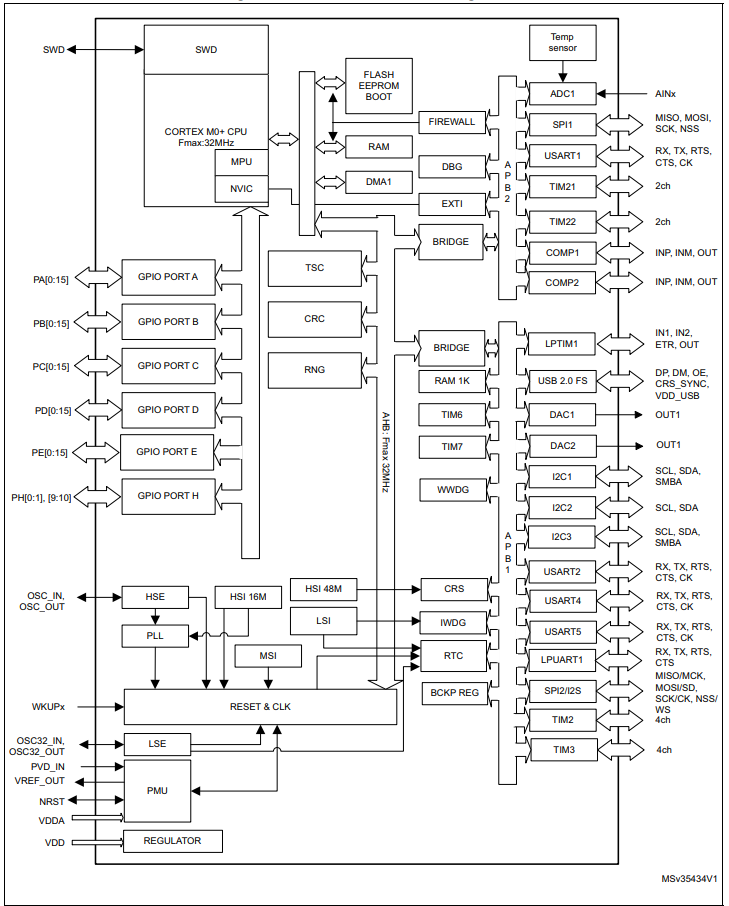
\includegraphics[ width = 0.8\textwidth]{HW_PART/Figs/stm32l072xx.png}
            \caption {Blokový diagram MCU STM32L072xx}
        \end{figure} 
    


\subsubsection{LoRa modul}
      $\text{LoRa}^{\text{TM}}$ je uzavřená technologie, kterou licencuje a vyvíjí firma SemTech. Všechny čipy podporující tuto modulaci nesou označení SX12xx a dělí se na dvě řady.\\
      První řada s čipy SX126x, SX127x, které se liší podle výkonosti nese označení \textit{LoRa Transceivers} je určená pro koncové uzly. Tyto čipy neumožňují multikanálový příjem paketů a jsou omezeny na využití jednoho SF (Spreading Factoru) v danou chvíli.\\
      Naproti tomu druhá řada s čipy SX125x, SX13xx s označením \textit{LoRa Gateways} je mnohem výkonnější a umožňuje automatickou detekci SF přijatého signálu.
      
       \question{Patří to sem???}
       
      Na trhu se nachází nepřeberné množství LoRa modulů, které se liší použitým LoRa čipem, tedy hlavně výstupním výkonem a parametry LoRa modulace a dále komunikačním rozhraním a cenou.\\
      Pro první prototyp měřicí jednotky byl nakonec použit LoRa modul přímo od firmy ST – \textbf{I-NUCLEO-SX1272D} s čipem SX1272, který byl součástí vývojářského kitu a který lze zapojit přímo do Nuclea.
      
      V druhé verzi a plošném spoji byl využit velmi rozšířený modul \textbf{RFM95W} s čipem SX1276, který se těší velké oblíbenosti především díky své nízké cenně.

    \textbf{Specifikace LoRa modulu RFM95W:}
        \begin{itemize}
            \item Celkový vysílací výkon až 161 dB
            \item Programovatelný bitrate až 300 kbps
            \item Citlivost až -148 dBm
            \item Proudový odběr ve SLEEP módu \SI{0.2}{\micro\ampere} 
            \item Proudový odběr ve RX módu kolem \SI{10}{\milli\ampere} 
            \item Proudový odběr ve TX módu \SI{29}{\milli\ampere} při RFOP +13 dBm
        \end{itemize}

     \begin{figure} [!h]
        \centering
        \begin{subfigure}[b]{0.6\textwidth}
             \centering
             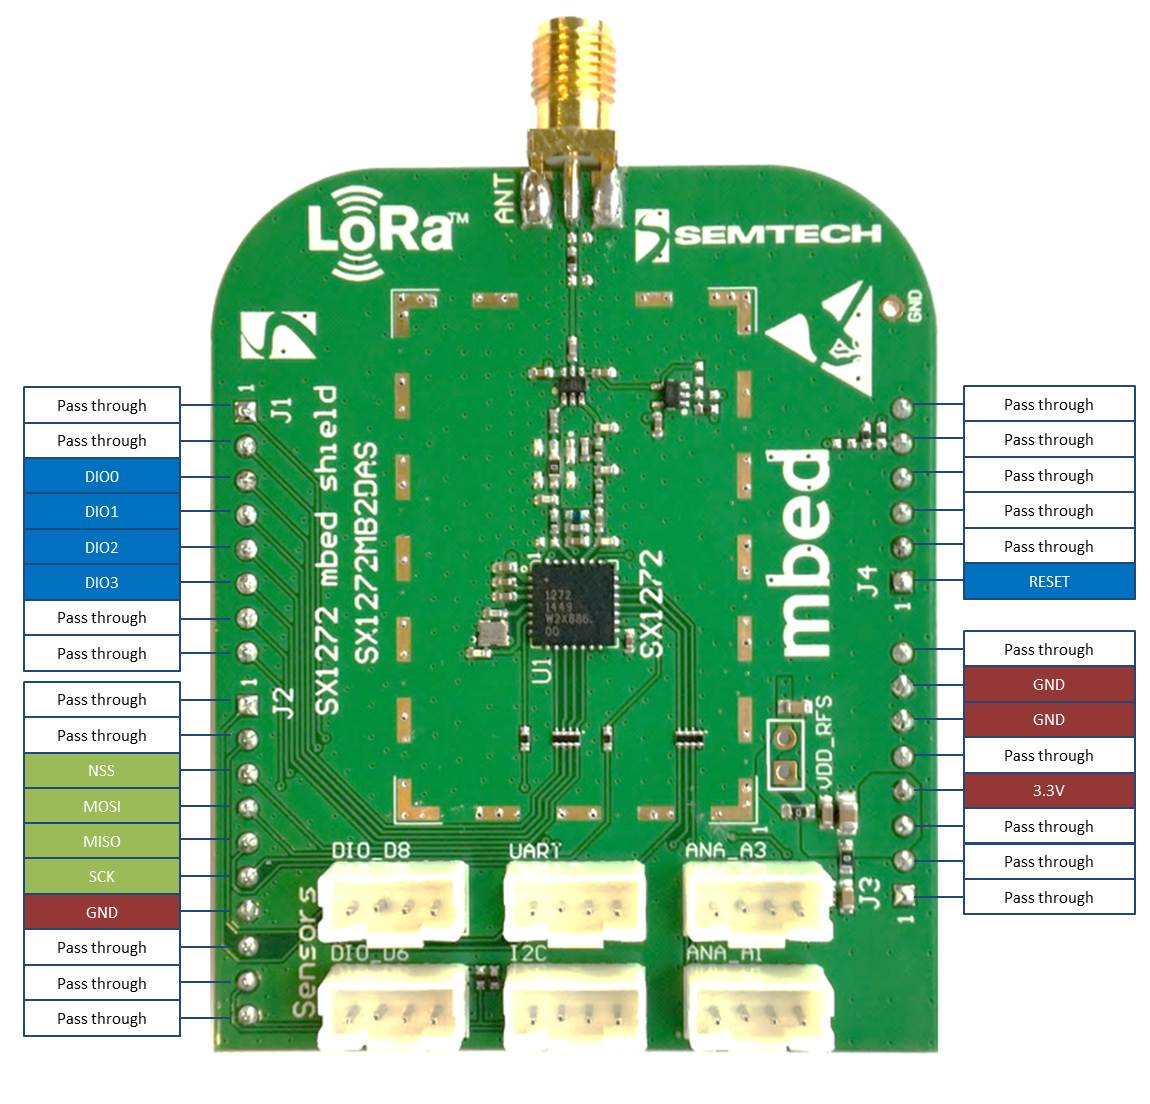
\includegraphics[width=\textwidth]{HW_PART/Figs/SX1272_pinout.jpg}
             \caption {LoRa modul I-NUCLEO-SX1272D}
             \label{fig:y equals x}
         \end{subfigure}
         \hfill
        \begin{subfigure}[b]{0.35\textwidth}
            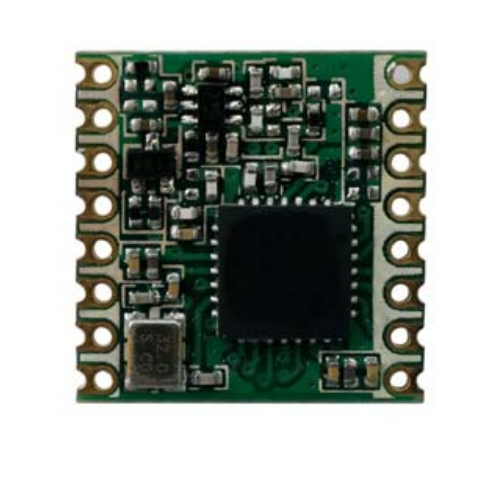
\includegraphics[ width =\textwidth]{HW_PART/Figs/rfm95W.png}
            \caption {LoRa modul RFM95W}
        \end{subfigure}
    \end{figure} 

\subsubsection{Senzor vibrací}
    Výběr akcelerometru byl ovlivněný vhodností pro detekci vibračních signálů a nízkou spotřebou. Tedy postačoval jednoosý akcelerometr s šířkou pásma kolem ... , čemuž vyhovoval akcelerometr \textbf{ADXL1002} od firmy Analog Devices. Tato řada akcelerometrů je přímo určena pro Condition monitoring.\\
    Tyto akcelerometry jsou navíc dodávané na vývojářské destičce  \textbf{EVAL-ADXL1002Z}, která je poměrně tlustá, odolná i vůči silným vibracím, dobře upevnitelná k samotným motorům, a je na ní také umístěn RC filtr, který zamezuje aliasingu.
    Analogový výstup akcelerometru je poté veden koaxiálním kabelem, jehož stínění potlačuje vliv vnějších rušivých polí na přenášený užitečný signál, a je poté zpracováván AD převodníkem na mikrokontroléru. 
    
    \todo{TASK: Refer to place where DSP is explained}
    
    \question{Specifikace koaxiálního kabelu? aktivní stínění?}
    
    \question{Jaký je běžný rozsah frekvenčních signálů a stačí jednoosý??, co je noise floor?}
    \question{Na co tam je RC filter vlastne - aliasing/sum?}

    \answer{rozsah, noise floor u analogového/ rozlišení u digitálního, šířka pásma/vzorkovací frekvence}

    \textbf{Specifikace akcelerometru ADXL1002:}
        \begin{itemize}
            \item Jednoosý akcelerometr typu MEMS (mikroelektromechanický)
            \item Šířka pásma $11 kHz$
            \item Měřicí rozsah $\pm50 g$
            \item Citlivost $40 mV/g$, při nulovém $g$ je na výstupu polovina napájecího napětí
            \item Analogový výstup
            \item Proudový odběr v měřícím módu \SI{1}{\milli\ampere}
            \item Proudový odběr v STDBY módu  \SI{225}{\micro\ampere} 
        \end{itemize}
        
    \begin{figure} [!hbp]
        \centering
        \begin{subfigure}[b]{0.6\textwidth}
             \centering
             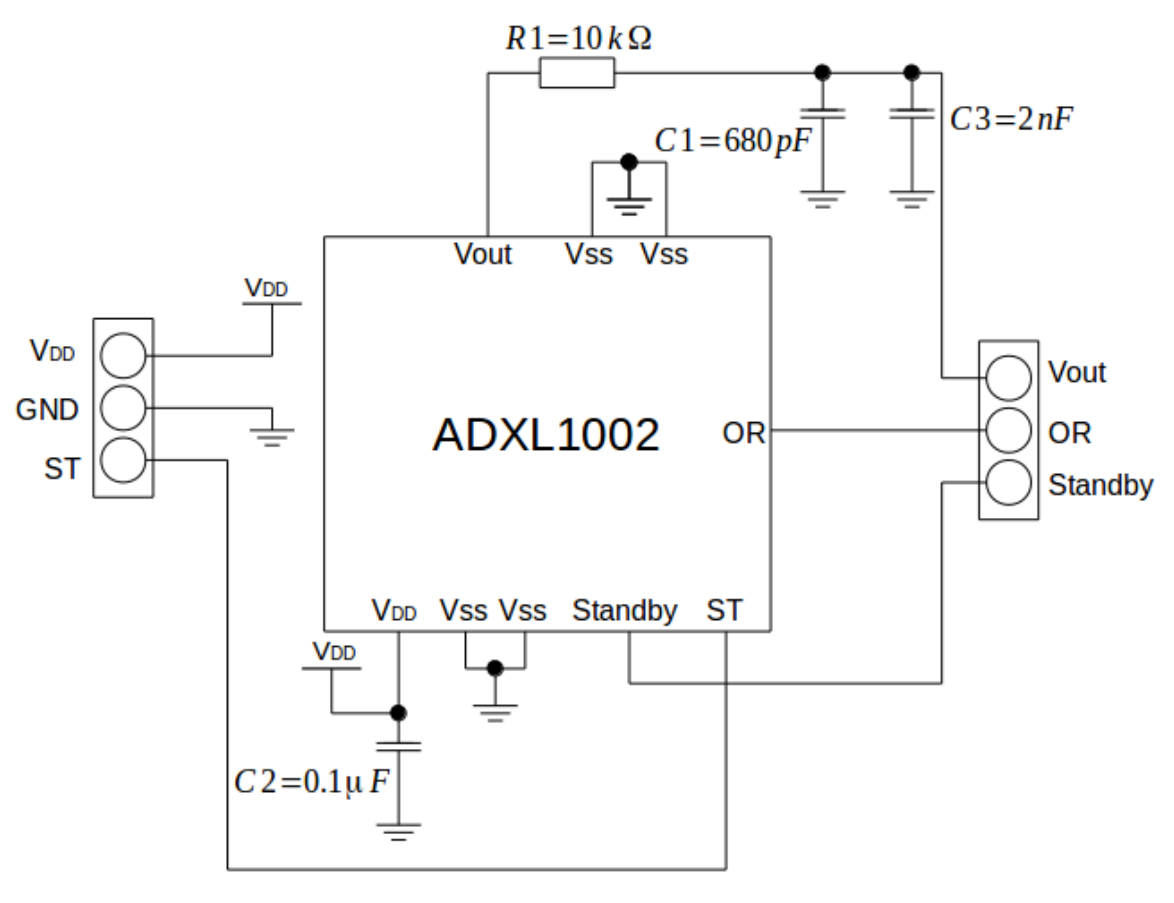
\includegraphics[width=\textwidth]{HW_PART/Figs/adxl1002.png}
             \caption {Schéma vývojové desky EVAL-ADXL1002Z}
             \label{fig:y equals x}
         \end{subfigure}
         \hfill
        \begin{subfigure}[b]{0.6\textwidth}
            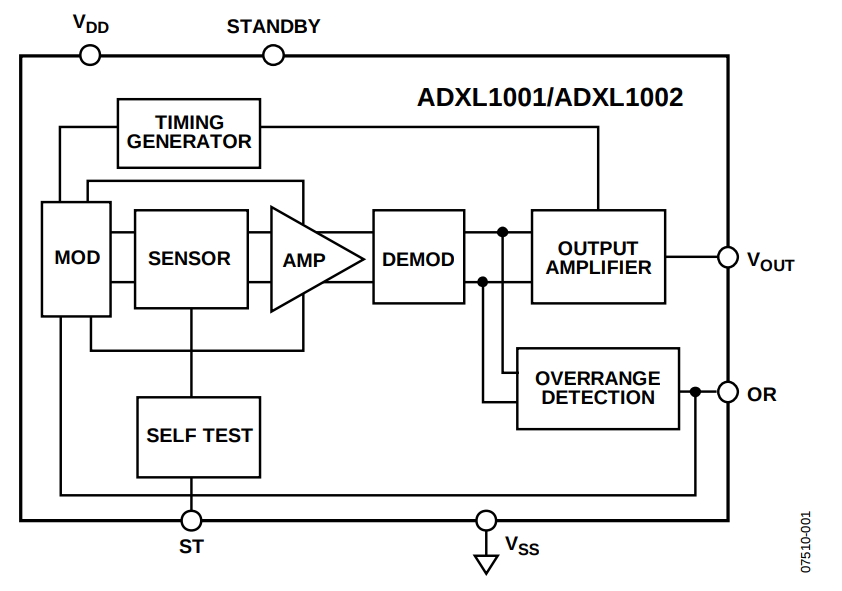
\includegraphics[ width =\textwidth]{HW_PART/Figs/adxl1002_functionaldiagram.png}
            \caption {Blokový diagram ADXL1002}
        \end{subfigure}
    \end{figure} 
    
    


\subsubsection{Teplotní senzor}
    Pro monitorování teploty bylo vybráno digitální teplotní čidlo \textbf{TMP75} od firmy Texas Instruments, které pro měření využívá 12bitový převodník. Jedná se o poměrně rozšířený senzor komunikující po I2C sběrnici, který je díky své malé spotřebě vhodný zejména do zařízení, které jsou poháněny baterií.

    \textbf{Specifikace teplotního čidla TMP75:}
        \begin{itemize}
            \item Přesnost $\pm$ \ang{1}C
            \item Programovatelné rozlišení 9-12 bitů
            \item Rozsah \ang{-40}C-\ang{+125}C
            \item Proudový odběr \SI{50}{\micro\ampere}
        \end{itemize}
     
     \begin{figure} [!hbp]
        \centering
        \begin{subfigure}[!h]{0.5\textwidth}
             \centering
             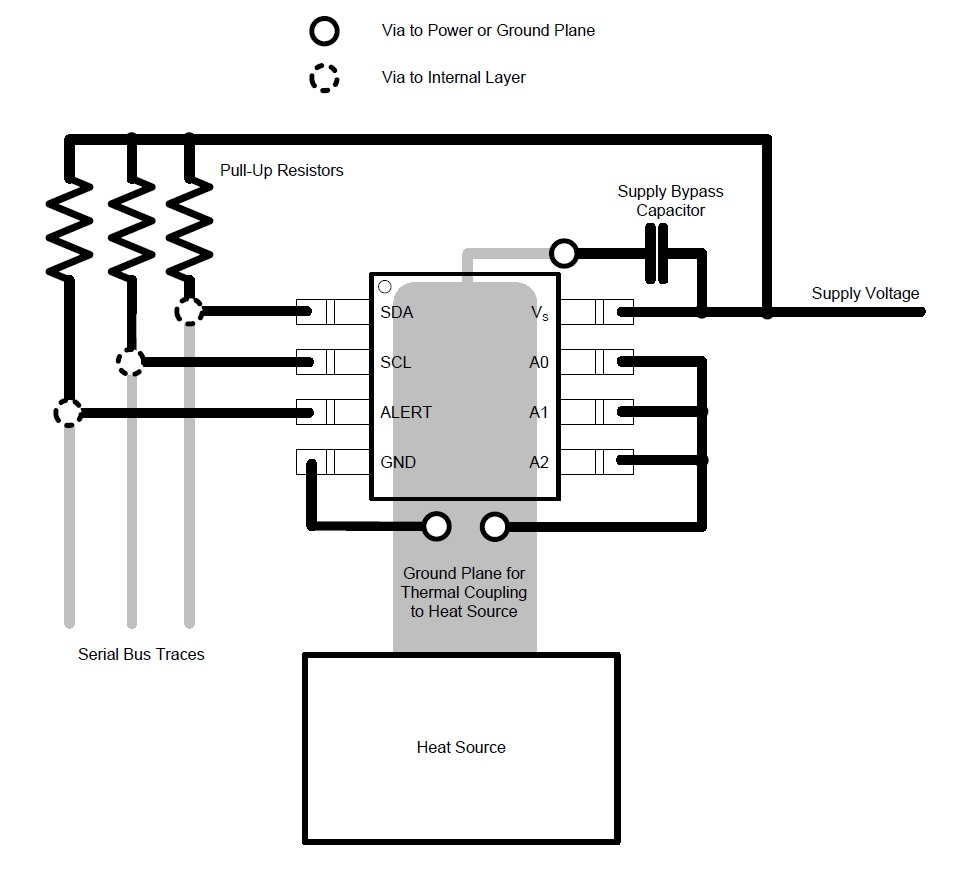
\includegraphics[width=\textwidth]{HW_PART/Figs/tmp75_connection.jpg}
             \caption {Schéma připojení TMP75}
         \end{subfigure}
         \hfill
        \begin{subfigure}[!h]{0.45\textwidth}
            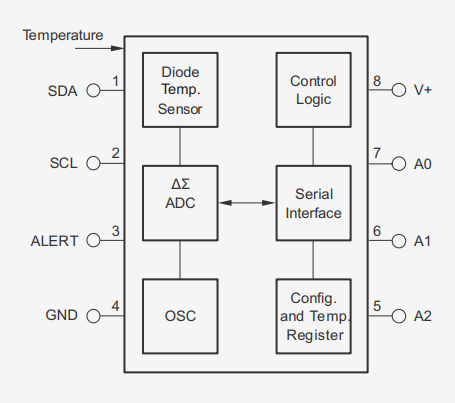
\includegraphics[ width =\textwidth]{HW_PART/Figs/tmp75_functionaldiagram.png}
            \caption {Blokový diagram TMP75}
        \end{subfigure}
    \end{figure} 

\subsection{Celkový design} 

\subsubsection{První prototyp}
    První verze měřicí jednotky byl vytvořen pomocí vývojářského kitu NUCLEO s procesorem STM32L073RZ, LoRa modulem s čipem SX1272 a nepájivým polem, do kterého byly připojeny vývody senzorů. Oba dva byly napájeny z Nuclea a byly k nim přidány kondenzátory pro blokování napájení. Výsledné zapojení lze vidět na obrázku.
    
    \todo{IMAGE: Make photo}
    
\subsection{Druhá verze}
    Druhá verze měřící jednotky byla vytvořena bez Nuclea zapájením čipu STM3272KZ na adaptor a připojením LoRa modulu RFM95W a senzorů na univerzální destičce...
    














\section{Řídicí jednotka (LoRa Gateway)}
\subsection{Výběr komponent}
\subsubsection{Mikrokontrolér (MCU)}

    Vlastní LoRa brána může být postavena spíše minimalisticky za použití určitého mikrokontroléru, tedy se slabým výkonem, ale nízkou cenou a spotřebou – například jako další STM32 jednotka s Ethernet nebo WiFi modulem nebo pomocí oblíbeného vývojářského čipu ESP8266/ESP32. Opačný přístup by bylo postavení brány s výpočetně silnějším počítačem a operačním systémem, tedy s velkým výkonem, ale vyšší cenou a spotřebou.
    Pro realizaci brány bylo ale nakonec použité \textbf{Raspberry Pi} verze 3 model B. 
    Motivací výběru Raspberry po zvážení kritérií popsaných výše byl zejména dostatečný výpočetní výkon, vývojářská podpora a výhody operačního systému. Spotřeba brány není tak důležité kritérium jako u koncových zařízení, protože brána může mít stálý zdroj napájení. Raspberry byl tedy jakýsi kompromis mezi výkonem a cennou.

\textbf{Specifikace Raspberry Pi model B:}
    \begin{itemize}
        \item 64 bitový čtyřjádrový procesor Broadcom BCM2837 1.2GHz, 1 GB RAM
        \item 40 externích GPIO pinů
        \item BCM43438 WLAN a Bluetooth Low Energy (BLE)
        \item 4 USB porty, HDMI, 3.5 mm jack
        \item Micro SD port
    \end{itemize}
    
\subsubsection{LoRa modul}
    Z důvodů popsaných v ... byla brána navržená jako jednokanálová. Pro LoRa komunikaci tedy nebylo nutné používat čipy ze série SX125x, SX13xx, a byl proto v obou verzích využit stejný čip jako u měřicí jednotky - SX1272 v první verzi a RFM95W ve druhé verzi.
    
\subsubsection{Displej}
    
 \subsubsection{První prototyp}
    První verze brány byla vytvořena pouze s LoRa modulem určeným původně pro Nucleo I-NUCLEO-SX1272D, který musel být s GPIO piny propojen jednotlivými drátky.
    
    \todo{IMAGE: Make picture of GW.}

 \subsubsection{Konečná verze}
 
 
 
 \question{TYPOGRAFIE - jednoty kurzivou nebo ne?}

\question{TYPOGRAFIE - pomlcky vs spojovniky}

\question{TYPOGRAFIE - stupen - mezera nebo ne}

\question{TYPOGRAFIE - mezery za jednotkami}
